\chapter{\protect\hyperlink{:}{量子力学、为什么我们需要量子场论}}
\addtocontents{toc}{\protect\hypertarget{:}{}}



\section{\protect\hyperlink{:}{量子力学}}
\addtocontents{toc}{\protect\hypertarget{:}{}}

量子力学是描述微观粒子运动规律的基本理论，它在解释原子、分子以及固体等系统的性质方面取得了巨大成功。然而，当我们试图将量子力学与狭义相对论结合起来时，遇到了严重的困难。此外，量子力学无法自然地处理粒子的产生和湮灭现象，而这在高能物理过程中是普遍存在的。这些困难促使我们发展出量子场论，它能够统一地描述粒子和场的量子行为。

\subsection{\protect\hyperlink{:}{为什么我们需要量子场论}}
\addtocontents{toc}{\protect\hypertarget{:}{}}

量子场论（Quantum Field Theory, QFT）是将量子力学与狭义相对论统一起来的理论框架。尽管量子力学在非相对论性领域取得了巨大的成功，但当我们试图将其推广到高能领域时，会遇到一些根本性的困难，这些困难正是我们需要量子场论的动机。

\subsubsection{\protect\hyperlink{:}{粒子数不守恒与粒子的产生湮灭}}

在量子力学中，系统的粒子数是固定的。然而，在高能物理实验中，粒子可以被产生和湮灭。例如：
\begin{itemize}
    \item 正负电子对湮灭产生光子：$e^+ + e^- \to \gamma + \gamma$
    \item 光子产生正负电子对：$\gamma \to e^+ + e^-$（在原子核附近）
    \item 高能碰撞中产生大量新粒子
\end{itemize}

量子力学无法自然地描述这类现象。量子场论通过将场进行量子化，引入产生算符 $\hat{a}^\dagger$ 和湮灭算符 $\hat{a}$，使得粒子数成为动力学变量，从而自然地描述了粒子的产生与湮灭。

\subsubsection{\protect\hyperlink{:}{相对论性量子力学的困难}}

将量子力学与狭义相对论结合的最早尝试是 Klein-Gordon 方程和 Dirac 方程。然而，这些"单粒子"相对论性方程都面临严重问题：

\begin{enumerate}
    \item \textbf{Klein-Gordon 方程的困难}：Klein-Gordon 方程 $\left(\partial_\mu\partial^\mu + m^2\right)\phi = 0$ 是关于时间的二阶微分方程，其概率密度可以取负值，无法解释为单粒子的几率密度。
    
    \item \textbf{Dirac 方程的困难}：Dirac 方程虽然给出了自旋 $\frac{1}{2}$ 粒子的正确描述，但其解中包含负能量态。为了解释这些负能量态，Dirac 提出了"狄拉克海"的概念，但这在概念上存在困难。
\end{enumerate}

量子场论通过将场本身作为量子化对象，而非单个粒子，从根本上解决了这些问题。负频率解被解释为反粒子的正频率解，粒子与反粒子的对称性自然出现。

\subsubsection{\protect\hyperlink{:}{全同粒子的统一描述}}

在量子力学中，玻色子和费米子需要分别处理，波函数的对称化或反对称化需要人为引入。量子场论通过场算符的对易关系（玻色子）或反对易关系（费米子），自动地给出了全同粒子的正确统计性质：

\begin{align*}
    \left[\hat{a}_i, \hat{a}_j^\dagger\right] &= \delta_{ij} \quad &\text{(玻色子)} \\
    \left\{\hat{c}_i, \hat{c}_j^\dagger\right\} &= \delta_{ij} \quad &\text{(费米子)}
\end{align*}

\subsubsection{\protect\hyperlink{:}{相互作用的自然描述}}

量子场论提供了描述粒子间相互作用的自然框架。相互作用通过在拉格朗日密度中引入场的耦合项来实现。例如，量子电动力学（QED）的相互作用拉格朗日密度为
\begin{equation*}
    \mathcal{L}_{\text{int}} = -e\bar{\psi}\gamma^\mu\psi A_\mu
\end{equation*}

其中 $\psi$ 是电子场，$A_\mu$ 是电磁场，$e$ 是耦合常数（电荷）。费曼图和微扰论的系统方法使得我们可以对物理过程进行精确计算。

\subsubsection{\protect\hyperlink{:}{总结}}

综上所述，量子场论是以下三方面需求的自然结果：
\begin{enumerate}
    \item 将量子力学与狭义相对论统一起来；
    \item 自然地描述粒子的产生与湮灭；
    \item 为基本相互作用提供统一的理论框架。
\end{enumerate}

量子场论不仅是粒子物理标准模型的数学语言，也是凝聚态物理中处理多体问题的重要工具。接下来，我们将从量子力学的场算符出发，逐步建立量子场论的基本框架。



\section{\protect\hyperlink{:}{场算符(Field operators)}}
\addtocontents{toc}{\protect\hypertarget{:}{}}

\subsection{\protect\hyperlink{:}{坐标与动量表象}}
\addtocontents{toc}{\protect\hypertarget{:}{}}

在此之前我们先回顾一下量子力学我们在描述一个态 $\ket{\alpha}$ 时可以使用坐标来描述 $\psi_\alpha(\vec{x}) = \braket{\vec{x}}{\alpha}$ 或者是用动量来描述 $\tilde{\psi}_\alpha(\vec{p}) = \braket{\vec{p}}{\alpha}$ 
\begin{equation*}
    \braket{\vec{p}}{\alpha} = \int d^3 x \braket{\vec{p}}{\vec{x}}\braket{\vec{x}}{\alpha}
\end{equation*}

接着在使用傅里叶变换
\begin{equation*}
    \tilde{\psi}_\alpha (\vec{p}) = \frac{1}{\sqrt{\mathcal{V}}} \int d^3 x e^{-i\vec{p}\cdot \vec{x}} \psi_\alpha (\vec{x})
\end{equation*}

因此 
\begin{equation*}
    \braket{\vec{p}}{\vec{x}} = \frac{1}{\sqrt{\mathcal{V}}} e^{-i\vec{p} \cdot \vec{x}}
\end{equation*}

如果 $\vec{p}$ 是离散的值时，其逆变换为
\begin{equation*}
    \psi_\alpha (\vec{x}) = \frac{1}{\sqrt{\mathcal{V}}} \sum_{\vec{p}} e^{i\vec{p}\cdot \vec{x}} \tilde{\psi}_\alpha (\vec{p})
\end{equation*}


\subsection{\protect\hyperlink{:}{简单谐振子(Simple harmonic oscillators)}}
\addtocontents{toc}{\protect\hypertarget{:}{}}
接下来回顾一下简单谐振子问题,其势能为 $\displaystyle \hat{V} = \frac{1}{2} K \hat{x}^2$ ,通过求解其薛定谔方程可以得到波函数
\begin{equation*}
    \psi_n(\xi) = \frac{1}{\sqrt{2^n n!}}\left(\frac{m\omega}{\pi \hbar}\right)^{1/4} H_n(\xi) e^{-\frac{1}{2}\xi^2} ,\qquad \xi = \sqrt{\frac{m\omega}{\hbar}}x
\end{equation*}

其中的 $\displaystyle H_n(\xi)$ 为厄密多项式，这里给出几幅波函数的图像
\begin{figure}[hbpt]
    \begin{minipage}{0.45\textwidth}
        \centering
        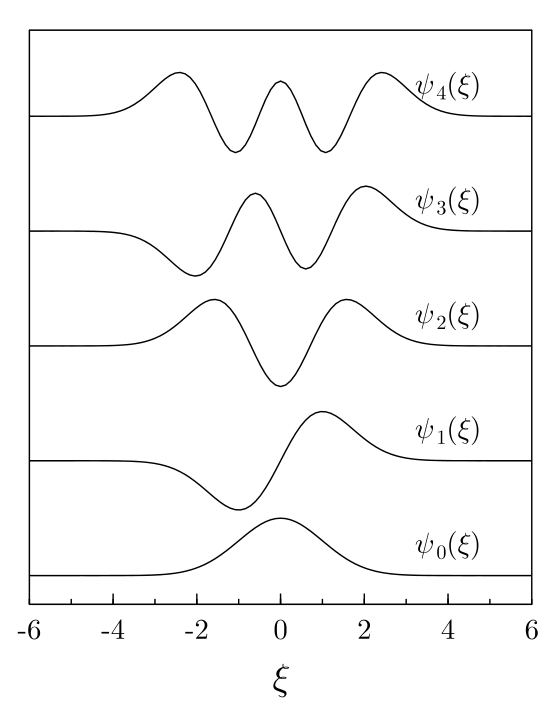
\includegraphics[width = 0.8\textwidth]{figure/一维简单谐振子解.png}
    \end{minipage}
    \hfill
    \begin{minipage}{0.45\textwidth}
        \centering
        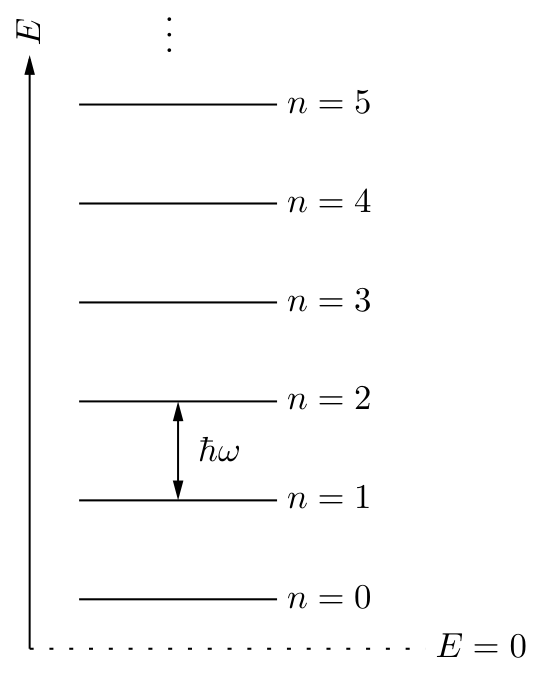
\includegraphics[width = 0.8\textwidth]{figure/一维简单谐振子能谱.png}
    \end{minipage}
\end{figure}

同时，其能谱（能量本征值）为 
\begin{equation*}
    E_n = \left(n + \frac{1}{2}\right)\hbar\omega
\end{equation*}

另外在求解过程当中我们还得到了一个所谓的频率 $\omega$ 并且将原来的常数 $K$ 进行了定义 $K\equiv m\omega^2$,于是哈密顿量重写为
\begin{equation*}
    \hat{H} = \frac{\hat{p}^2}{2m} + \frac{1}{2} m \omega^2 \hat{x}^2
\end{equation*}

似乎我们可以根据平方差写成这样的形式
\begin{equation*}
    \frac{1}{2} m \omega^2\left(\hat{x} - \frac{i}{m\omega}\hat{p}\right)\left(\hat{x} + \frac{i}{m\omega}\hat{p}\right)
\end{equation*}

但是将其展开所得到的为
\begin{equation*}
    \frac{\hat{p}^2}{2m} + \frac{1}{2} m \omega^2 \hat{x}^2 - \frac{1}{2}\hbar\omega = \hat{H} - \frac{1}{2}\hbar\omega
\end{equation*}

这相差的 $\displaystyle \frac{1}{2}\hbar\omega $ 是由于要修正零点能

在这里，算符 $\hat{x},\hat{p}$ 是厄密的，而算符 $\displaystyle \hat{x} - \frac{i}{m\omega}\hat{p}$ 与算符 $\displaystyle \hat{x} + \frac{i}{m\omega}\hat{p}$ 是互相自伴的，这也导致这两个新的算符是非厄密的，因此无法将其联系到任何的可观测量，我们给这两个算符进行重新定义，得到了所谓的产生和湮灭算符 $\hat{a}^\dagger,\hat{a}$
\begin{align*}
    \hat{a}^\dagger = \sqrt{\frac{m\omega}{2\hbar}}\left(\hat{x} - \frac{i}{m\omega}\hat{p}\right) \\
    \hat{a} = \sqrt{\frac{m\omega}{2\hbar}}\left(\hat{x} + \frac{i}{m\omega}\hat{p}\right)
\end{align*}

通过计算我们可以得到以下几个关系式
\begin{align*}
    \left[\hat{a},\hat{a}^\dagger\right] &= 1 \\
    \hat{x} &= \sqrt{\frac{\hbar}{2m\omega}} \left(\hat{a} + \hat{a}^\dagger\right) \\
    \hat{p} &= -i\sqrt{\frac{\hbar m \omega}{2}} \left(\hat{a} - \hat{a}^\dagger\right) \\
    \hat{H} &= \hbar \omega \left(\hat{a}^\dagger \hat{a} + \frac{1}{2}\right)
\end{align*}


如果我们设算符 $\hat{a}^\dagger \hat{a}$ 有本征值为 $n$ 的本征态 $\ket{n}$ 那么相应的谐振子的哈密顿量也会有相应的本征值为 $\hbar \omega \left(\frac{1}{2} + n\right)$ 的本征态 $\ket{n}$ 这刚刚好和我们算到的能量本征值 $E_n = \hbar \omega \left(\frac{1}{2} + n\right)$ 对应上，接下来我们只需要证明一下 $n$ 取非零整数即可，关于其非负性容易证明
\begin{equation*}
    n = \bra{n}\hat{a}^\dagger\hat{a}\ket{n} = \left|\hat{a}\ket{n}\right|^2 \geqslant  0
\end{equation*}


\subsection{\protect\hyperlink{:}{占有数表象(Occupation number representation)}}
\addtocontents{toc}{\protect\hypertarget{:}{}}

在这里为了方便起见，我们用别的符号来定义一下这个算符，并且命名为粒子数算符(number operator)
\begin{equation*}
    \hat{n} = \hat{a}^\dagger \hat{a}
\end{equation*}


这样就有
\begin{equation*}
    \hat{n}\ket{n} = n\ket{n}
\end{equation*}


然后就是这些关系，这里不做证明，证明很简单，大家可以自己尝试一下
\begin{align*}
    \hat{n}\hat{a}^\dagger\ket{n} &= \left(n + 1\right) \hat{a}^\dagger\ket{n} \\
    \hat{n}\hat{a}\ket{n} &= \left(n - 1\right) \hat{a}\ket{n} \\
    \hat{a}^\dagger \ket{n} &= \sqrt{n + 1}\ket{n + 1} \\
    \hat{a} \ket{n} &= \sqrt{n} \ket{n}
\end{align*}

很显然，我们的湮灭算符 $\hat{a}$ 可以使简单谐振子的能级下降一级，而我们的产生算符 $\hat{a}^\dagger$ 可以使简单谐振子的能级增加一级，因此如果我们不断地对一个本征态 $\ket{n}$ 作用上湮灭算符 $\hat{a}$ ，那么最终将会降到基态（真空态）$\ket{0}$ ,在这里我们规定：当湮灭算符作用到基态时，为 $0$，即 $\displaystyle \hat{a}\ket{0} = 0$,在这个规定下，我们的哈密顿量在基态的能量本征值为
\begin{equation*}
    \hat{H} \ket{0} = \hbar\omega \left(\hat{n} + \frac{1}{2}\right) \ket{0} = \frac{1}{2}\hbar\omega \ket{0}
\end{equation*}

可以看到这时候的基态就是我们的零点能。

另外，我们也可以不断地对某个态作用上产生算符 $\hat{a}^\dagger$ ，最终我们可以得到第 $n$ 能级的态矢量
\begin{equation*}
    \ket{n} = \frac{\left(\hat{a}^\dagger\right)^n}{\sqrt{n!}}\ket{0}
\end{equation*}

接下来考虑更为一般的情况，哈密顿量为很多独立的哈密顿量的总和
\begin{equation*}
    \hat{H} = \sum_{k = 1}^{N} \hat{H}_k =\sum_{k = 1}^{N} \left(\frac{\hat{p}_k^2}{2m_k} + \frac{1}{2} m_k \omega_k^2 \hat{x}_k^2\right)
\end{equation*}

我们将此时的态矢量记作每一个能级上的粒子数量的个数，例如
\begin{equation*}
    \ket{n_1,n_2,\cdots,n_k,\cdots}
\end{equation*}

当我们的产生湮灭算符作用到这些态上时将会是这样的效果
\begin{align*}
    \hat{a}_k^\dagger \ket{n_1,n_2,\cdots,n_k,\cdots} &\propto \ket{n_1,n_2,\cdots,n_k + 1,\cdots} \\
    \hat{a}_k \ket{n_1,n_2,\cdots,n_k,\cdots} &\propto \ket{n_1,n_2,\cdots,n_k - 1,\cdots}
\end{align*}

而对于这些升降算符有这样的对易关系
\begin{align*}
    \left[\hat{a}_k,\hat{a}_q\right] &= \left[\hat{a}_k^\dagger,\hat{a}_q^\dagger\right] = 0 \\
    \left[\hat{a}_k,\hat{a}_q^\dagger\right] &= \delta _{kq}
\end{align*}

此时的哈密顿量也可以像之前的简单谐振子问题一样，写成
\begin{equation*}
    \hat{H} = \sum_{k=1}^{N} \hbar\omega_k \left(\hat{a}_k^\dagger \hat{a}_k + \frac{1}{2}\right)
\end{equation*}

同时我们定义真空态（基态）为 $\displaystyle \ket{0,0,0,\cdots}$,也同样有
\begin{equation*}
    \hat{a}_k \ket{0,0,0,\cdots} = 0
\end{equation*}

而产生算符也有和简单谐振子的相似性质
\begin{equation*}
    \ket{n_1,n_2,\cdots,n_N} = \frac{1}{\sqrt{n_1! n_2! \cdots n_N!}}\left(\hat{a}_1^\dagger\right)^{n_1}\left(\hat{a}_2^\dagger\right)^{n_2}\cdots\left(\hat{a}_N^\dagger\right)^{n_N} \ket{0,0,0,\cdots}
\end{equation*}

简单记作
\begin{equation*}
    \ket{\left\{n_k\right\}} = \prod_k \frac{1}{\sqrt{n_k!}}\left(\hat{a}_k^\dagger\right)^{n_k}\ket{0}
\end{equation*}

在这里，我们所讨论的其实一直是在谐振子背景下产生量子，但不应该仅仅只在谐振子问题下，还应该让粒子在一个特定的动量态(momentum state) $\ket{p_m}$ ,因此我们将下标 $k$ 改为下标 $p_m$ 以此来表示在特定的 momentum state 下的算符，但是这一步操作仍然需要很谨慎的进行，接下来举个例子

\begin{example}
    给定一个双粒子体系其 momentum states 分别为 $p_1,p_2$ ，那么在 Occupation number representation 下，态矢量表示为 $\ket{n_1,n_2}$,我们做如下定义
    \begin{equation*}
        \hat{a}_{p_1}^\dagger \ket{00} = \ket{10} ,\quad \hat{a}_{p_2}^\dagger \ket{00} = \ket{01}
    \end{equation*}

    根据这个定义，我们有 
    \begin{equation*}
        \hat{a}_{p_2}^\dagger\hat{p_1}^\dagger \ket{0} \propto \ket{11} ,\quad \hat{a}_{p_1}^\dagger\hat{p_2}^\dagger \ket{0} \propto \ket{11}
    \end{equation*}

    这也就是说 
    \begin{equation*}
        \hat{a}_{p_2}^\dagger\hat{p_1}^\dagger = \lambda \hat{a}_{p_1}^\dagger\hat{p_2}^\dagger
    \end{equation*}

    在这里，我们假设 $\lambda = \pm 1$ 至于别的情况我们之后再说，这里的假设将会导致波函数出现对称和反对称两种情况
    \begin{enumerate}
        \item[case 1] $\lambda = 1$ ，我们将这时候的粒子称为玻色子
        \begin{equation*}
            \hat{a}_{p_2}^\dagger\hat{p_1}^\dagger = \hat{a}_{p_1}^\dagger\hat{p_2}^\dagger
        \end{equation*}

        根据这个式子我们知道对易关系
        \begin{equation*}
            \left[\hat{a}_i^\dagger,\hat{a}_j^\dagger\right] = 0
        \end{equation*}

        当然对于不同的态的产生湮灭算符之间的对易关系为
        \begin{equation*}
            \left[\hat{a}_i,\hat{a}_j^\dagger\right] = \delta_{ij}
        \end{equation*}

        对其任意的一个态矢量，可以这样表示
        \begin{equation*}
            \ket{n_1,n_2,n_3,\cdots} = \prod_m \frac{1}{\left(n_{p_m}!\right)^{\frac{1}{2}}}\left(\hat{a}_{p_m}^\dagger\right)^{n_{p_m}} \ket{0}
        \end{equation*}

        由于我们知道，对于玻色子，不同的量子态 $\ket{n_{p_m}},\ket{n_{p_q}}$ 其产生算符是可以对易的，这也导致了
        \begin{equation*}
            \hat{a}_{p_1}^\dagger \hat{a}_{p_2}^\dagger \ket{0} = \hat{a}_{p_2}^\dagger \hat{a}_{p_1}^\dagger \ket{0} = \ket{1_{p_1},1_{p_2}}
        \end{equation*}

        这也就是说不论我按照什么顺序去放置粒子，都是一样的效果。（原文：it doesn’t matter which order you put particles in the states,you get exactly the same in either case）

        同时，总的来说我们可以有
        \begin{align*}
            \hat{a}_i^\dagger \ket{n_1,n_2,\cdots,n_i,\cdots} &= \sqrt{n_i + 1} \ket{n_1,n_2,\cdots,n_i +1 ,\cdots} \\
            \hat{a}_i \ket{n_1,n_2,\cdots,n_i,\cdots} &= \sqrt{n_i} \ket{n_1,n_2,\cdots,n_i -1 ,\cdots}
        \end{align*}

        \item[case 2] $\lambda = -1$ ，我们将这时候的粒子称为费米子
        
        首先我们写出费米子的产生算符为 $\hat{c}_i^\dagger$ 这是为了和玻色子做一个区分，并且我们发现其存在反对易关系
        \begin{equation*}
            \left\{\hat{c}_i^\dagger,\hat{c}_j^\dagger\right\} \equiv \hat{c}_i^\dagger \hat{c}_j^\dagger + \hat{c}_j^\dagger\hat{c}_i^\dagger = 0
        \end{equation*}
        
        这也将导出
        \begin{equation*}
            \hat{c}_i^\dagger \hat{c}_i^\dagger + \hat{c}_i^\dagger\hat{c}_i^\dagger = 0 \quad\Rightarrow \hat{c}_i^\dagger \hat{c}_i^\dagger = 0
        \end{equation*}

        这其中的意思是，当你尝试将两个费米子强行放在同一个态的话，他们会立刻发生湮灭，这也就是 Pauli exclusion principle ，这里给出原文
        \begin{theorem}[Pauli exclusion principle]
            Each state can either be unoccupied or contain a single fermion.
        \end{theorem}

        同时我们还有反对易关系
        \begin{align*}
            \left\{\hat{c}_i,\hat{c}_j\right\} &= 0 \\
            \left\{\hat{c}_i,\hat{c}_j^\dagger\right\} &= \delta_{ij}
        \end{align*}

        与玻色子不同的是，当我们用不同的顺序去放置粒子，这将导致不一样的结果.It really does matter which order you put the particles into the states.

        总的来说我们可以有
        \begin{align*}
            \hat{c}_i^\dagger \ket{n_1,n_2,\cdots,n_i,\cdots} &= \left(-1\right)^{\sum_i} \sqrt{1 - n_i} \ket{n_1,n_2,\cdots,n_i +1 ,\cdots} \\
            \hat{c}_i \ket{n_1,n_2,\cdots,n_i,\cdots} &= \left(-1\right)^{\sum_i} \sqrt{n_i} \ket{n_1,n_2,\cdots,n_i -1 ,\cdots} \\
            \sum_i &= n_1 + n_2 + \cdots + n_{i - 1}
        \end{align*}
        
    \end{enumerate}
\end{example}

刚刚说的都是离散的情况，对于连续的情况我们直接写成
\begin{align*}
    \left[\hat{a}_{\vec{p}},\hat{a}_{\vec{q}}^\dagger\right] &= \delta^{(3)}\left(\vec{p} - \vec{q}\right) \\
    \hat{H} &= \int d^3p E_{\vec{p}} \  \hat{a}_{\vec{p}}^\dagger \  \hat{a}_{\vec{p}}
\end{align*}

这就是所谓的连续极限.



\subsection{\protect\hyperlink{:}{场算符的诞生}}
\addtocontents{toc}{\protect\hypertarget{:}{}}

在前面的内容当中，我们使用到了产生算符 $\hat{a}_{\vec{p}}^\dagger$ 和湮灭算符 $\hat{a}_{\vec{p}}$，但是当我们有一个真空态，并且使用一个产生算符 $\hat{a}_{\vec{p}}^\dagger$ 作用在它的上面，那么我们将会得到一个态 $\hat{a}_{\vec{p}}^\dagger$ 其包含有一个在动量空间 $\vec{p}$ 的单粒子，但是尽管动量本征态在空间当中被展开，但也仅仅是在动量空间中，现在我们将通过算符的线性组合以及傅里叶变换来生成算符，而我们现在需要的就是场算符(field operators) ，而场算符便是在空间位置产生或湮灭粒子，因此我们将场算符定义为
\begin{equation*}
    \hat{\psi}^\dagger (\vec{x}) = \frac{1}{\sqrt{\mathcal{V}}}\sum_{\vec{p}} \hat{a}_{\vec{p}}^\dagger e^{-i\vec{p}\cdot \vec{x}}
\end{equation*}

这个算符将会在位置 $\vec{x}$ 产生一个粒子。同时我们也可以定义湮灭场算符
\begin{equation*}
    \hat{\psi} (\vec{x}) = \frac{1}{\sqrt{\mathcal{V}}}\sum_{\vec{p}} \hat{a}_{\vec{p}} e^{i\vec{p}\cdot \vec{x}}
\end{equation*}

接下来，我们来尝试下吧
\begin{example}
    给出一个量子态 $\ket{\Psi} = \hat{\psi}^\dagger (\vec{x})\ket{0}$ 并检验一下它是否确定对应于一个特定位置的单粒子
    \begin{equation*}
        \ket{\Psi} = \hat{\psi}^\dagger (\vec{x}) \ket{0} = \frac{1}{\sqrt{\mathcal{V}}} \sum_{\vec{p}} e^{-i\vec{p}\cdot\vec{x}} \hat{a}_{\vec{p}}^\dagger \ket{0}
    \end{equation*}

    为了计算出这个态的粒子数量，我们将使用占有数算符 $\hat{n}_{\vec{p}}$ 作用到这个态上，即 
    \begin{equation*}
        \sum_{\vec{q}} \hat{n}_{\vec{q}} \ket{\Psi} = \frac{1}{\sqrt{\mathcal{V}}} \sum_{\vec{q}\vec{p}} e^{-i\vec{p}\cdot\vec{x}} \hat{a}_{\vec{p}}^\dagger \hat{a}_{\vec{p}} \hat{a}_{\vec{p}}^\dagger \ket{0}
    \end{equation*}

    我们知道 $\bra{0} \hat{a}_{\vec{p}} \hat{a}_{\vec{p}}^\dagger \ket{0}  = \delta_{\vec{q}\vec{p}}$,于是有
    \begin{equation*}
        \sum_{\vec{q}} \hat{n}_{\vec{q}} \ket{\Psi} = \ket{\Psi}
    \end{equation*}

    这也就是说 $\ket{\Psi}$ 就是特征值为 $1$ 的占有数算符的特征态

    为了找到确切的粒子产生的位置，我们先定义 $\ket{\vec{p}} = \hat{a}_{\vec{p}}^\dagger \ket{0}$ 接下来我们就将另外一个位置本征矢 $\ket{\vec{y}}$ 作用到 $\ket{\Psi}$ 上 
    \begin{align*}
        \braket{\vec{y}}{\Psi} &= \bra{\vec{y}}\hat{\psi}^\dagger(\vec{x}) \ket{0} \\
        &= \frac{1}{\sqrt{\mathcal{V}}}\sum_{\vec{p}}e^{-i \vec{p}\cdot \vec{x}}\braket{\vec{y}}{\vec{p}} \\
        &= \frac{1}{\mathcal{V}} \sum_{\vec{p}}e^{-i\vec{p} \cdot \left(\vec{x} - \vec{y}\right)} \\
        &= \delta^{(3)}\left(\vec{x} - \vec{y}\right)
    \end{align*}

    这也就是说，这个产生的粒子，只有当 $\vec{y} = \vec{x}$ 时才能被找到
\end{example}

此外还有这些性质
\begin{align*}
    \left[\hat{\psi}(\vec{x}) , \hat{\psi}^\dagger(\vec{y})\right] &= \delta^{(3)} \left(\vec{x} - \vec{y}\right) \\
    \left[\hat{\psi}(\vec{x}) , \hat{\psi}(\vec{y})\right]&= \left[\hat{\psi}^\dagger(\vec{x}) , \hat{\psi}^\dagger(\vec{y})\right] = 0 \\
    \left\{\hat{\psi}(\vec{x}) , \hat{\psi}^\dagger(\vec{y})\right\} &= \delta^{(3)} \left(\vec{x} - \vec{y}\right) \\
    \left\{\hat{\psi}^\dagger(\vec{x}) , \hat{\psi}^\dagger(\vec{y})\right\} &= \left\{\hat{\psi}(\vec{x}) , \hat{\psi}(\vec{y})\right\} = 0
\end{align*}




场是被定义在所有时间空间点上的$(\vec{x},t)$,记作$$\phi_a(\vec{x},t)$$


尽管在经典力学中我们描述一个有限维空间中的粒子的广义坐标为$q_a(t)$,但是$\phi_a(\vec{x},t)$中，这里的$a$和$\vec{x}$仅仅是一个符号而已，我们所讨论的场，是具有无限自由度的







\subsection{\protect\hyperlink{:}{场的动力学与举例}}
\addtocontents{toc}{\protect\hypertarget{:}{}}

\subsubsection{\protect\hyperlink{:}{电磁场}}
\addtocontents{toc}{\protect\hypertarget{:}{}}

在经典物理当中，最好的例子应该就是电场$E(\vec{x},t)$和磁场$B(\vec{x},t)$了,并且，我们在电动力学当中，利用这两个场所定义出来的标势$\phi$和矢势$\vec{A}$将这两个三矢量合并为了一个四分量场$A_\mu(\phi,\vec{A})$,且电场和磁场可以由标势和矢势给出
\begin{align*}
    \vec{E}=-\nabla\phi-\frac{\partial\vec{A}}{\partial t}\quad\quad\vec{B}=\nabla\times\vec{A}
\end{align*}

同时还需要两个麦克斯韦方程组中的内容进行规定
\begin{align*}
    \nabla\cdot\vec{B}=0\quad\quad\frac{\partial}{\partial t}\vec{B}=-\nabla\times\vec{E}
\end{align*}



\subsection{\protect\hyperlink{:}{拉格朗日场论}}
\addtocontents{toc}{\protect\hypertarget{:}{}}

在之前的经典力学的复习当中，我们给出了一个系统的拉格朗日量与作用量的关系
\[S=\int dt L(q,\dot{q},t)\]

在场论当中，拉格朗日量是以$\phi,\nabla\phi$作为变量的，同时为了和别的四矢量进行统一，我们需要改变一下拉格朗日量的形式，即
\begin{equation*}
    L=\int d^3x\mathcal{L}(\phi,\partial_\mu\phi)
\end{equation*}

于是作用量将被写成
\begin{align*}
    S&=\int dt\int d^3x\mathcal{L}(\phi,\partial_\mu\phi)\\
    &=\int d^4x \mathcal{L}(\phi,\partial_\mu\phi)
\end{align*}

作用量显然是关于场算符$\phi$的泛函，最小作用量原理表明，当系统在四维空间演化时，在所有可能的演化中，符合物理真实动力学的演化路径应当是使得作用量取最小的路径，因此，我们考虑泛函$S[\phi]$的变分为$0$。
\begin{align*}
    0&=\delta S[\phi]\\
    &=\int d^4x \left\{\frac{\partial\mathcal{L}}{\partial \phi}\delta\phi+\frac{\partial \mathcal{L}}{\partial(\partial_\mu \phi)}\delta(\partial_\mu \phi)\right\}\\
    &=\int d^4x \left\{\textcolor{blue}{\frac{\partial\mathcal{L}}{\partial \phi}\delta \phi-\partial_\mu\left(\frac{\partial \mathcal{L}}{\partial(\partial_\mu\phi)}\right)\delta \phi}+\textcolor{red}{\partial_{\mu}\left(\frac{\partial \mathcal{L}}{\partial(\partial_\mu\phi)}\delta\phi\right)}\right\}
\end{align*}

这其中的第三项（也就是标红的部分）可以转化为四维时空积分区域的边界上的表面积分，一般场在其边界处为$0$,这也就是在告诉我们$\delta \phi=0$,因此这一项将会消失，但为了使得作用量的变分恒为$0$,我们就必须要让蓝色的部分为$0$,于是，我们得到了经典场的运动方程
\begin{equation*}
    \partial_\mu\left(\frac{\partial \mathcal{L}}{\partial(\partial_\mu\phi)}\right)-\frac{\partial\mathcal{L}}{\partial \phi}=0
\end{equation*}

如果拉格朗日量当中有多个场，那么对于每个场都有一个这样的方程与之对应。


\subsection{\protect\hyperlink{:}{哈密顿场论}}
\addtocontents{toc}{\protect\hypertarget{:}{}}

在离散系统里面，我们给每一个广义坐标都对应的定义了一个广义动量（又被称为共轭动量）$p(\vec{x})\equiv\frac{\partial L}{\partial \dot{q}}$，于是哈密顿量$H\equiv\sum p\dot{q}-L$在场论当中，我们假装空间点$\vec{x}$是离散的间隔，于是可以定义出
\begin{align*}
    p(\vec{x})&\equiv\frac{\partial L}{\partial \phi(\vec{x})}\\
    &=\frac{\partial}{\partial \phi(\vec{x})}\int\mathcal{L}(\phi(\vec{y}),\partial_\mu\phi(\vec{y}))d^3y\\
    &\sim \frac{\partial}{\partial \phi(\vec{x})}\sum_{\vec{y}}\mathcal{L}(\phi(\vec{y}),\partial_\mu\phi(\vec{y}))d^3y\\
    &=\pi(\vec{x})d^3x
\end{align*}

其中
\begin{align*}
    \pi(\vec{x})=\frac{\partial \mathcal{L}}{\partial \partial_\mu\phi(\vec{x})}
\end{align*}

这个就是$\phi(\vec{x})$的\textbf{共轭动量密度}。于是哈密顿量写作
\begin{align*}
    H=\sum p(\vec{x})\partial_\mu\phi(\vec{x})-L
\end{align*}

将其推广至连续的情况，即
\begin{align*}
    H&=\int d^3x \left[\pi(\vec{x})\dot{\phi}(\vec{x})-\mathcal{L}\right]\\
    &=\int d^3x \mathcal{H}
\end{align*}

其中，$\mathcal{H}$被称之为哈密顿密度。


在讲完了这两个场理论之后，我们将举一个简单的实标量场$\phi(\vec{x},t)$，他的拉格朗日量可以写为
\begin{align*}
    \mathcal{L}&=\frac{1}{2}\eta^{\mu\nu}\partial_\mu\phi\partial_\nu\phi-\frac{1}{2}m^2\phi^2\\
    &=\frac{1}{2}\dot{\phi}^2-\frac{1}{2}(\nabla \phi)^2-\frac{1}{2}m^2\phi^2
\end{align*}

将其带入到拉格朗日方程当中，
\begin{align*}
    \partial_\mu\left(\frac{\partial(\frac{1}{2}\eta^{\mu\nu}\partial_\mu\phi\partial_\nu\phi-\frac{1}{2}m^2\phi^2)}{\partial(\partial_\mu\phi)}\right)&=\frac{\partial(\frac{1}{2}\eta^{\mu\nu}\partial_\mu\phi\partial_\nu\phi-\frac{1}{2}m^2\phi^2)}{\partial \phi}\\
    \left(\partial^\mu\partial_\mu+m^2\right)\phi&=0\\
    \left(\frac{\partial^2}{\partial t^2}-\nabla^2+m^2\right)\phi&=0
\end{align*}

这个例子所计算出来的便是大名鼎鼎的Klein-Gordon 方程。

同时，这个例子当中，可以看出这个场的动能项$T$为
\begin{align*}
    T=\int d^3x\frac{1}{2}\dot{\phi}^2
\end{align*}

场的势能项$V$为
\begin{align*}
    V=\int d^3x \left(\frac{1}{2}(\nabla\phi)^2+\frac{1}{2}m^2\phi^2\right)
\end{align*}

此外，还可以计算出共轭动量密度
\begin{align*}
    \pi(\vec{x})=\frac{\partial\mathcal{L}}{\partial\dot{\phi}}=\dot{\phi}(\vec{x})
\end{align*}

于是，可以得出哈密顿密度
\begin{align*}
    \mathcal{H}=\pi\dot{\phi}-\mathcal{L}=\frac{1}{2}\dot{\phi}^2+\frac{1}{2}(\nabla\phi)^2+\frac{1}{2}m^2\phi^2
\end{align*}

写为哈密顿量就是
\begin{align*}
    H=\int d^3x \mathcal{H}=\int d^3x \left(\frac{1}{2}\dot{\phi}^2+\frac{1}{2}\left(\nabla\phi\right)^2+\frac{1}{2}m^2\phi^2\right)
\end{align*}

这三项中，第一项是时间中移动的能量、第二项是空间中切变的能量、最后一项是场本身的能量

\section{\protect\hyperlink{:}{Lorentz Invariance}}
\addtocontents{toc}{\protect\hypertarget{:}{}}


之前的经典力学当中只是比较草率地讲解了一点点洛伦兹变换,这一次则是希望可以将洛伦兹变换进行一次系统的讲解。
\begin{align*}
    \varLambda_\nu^\mu\to
    \begin{pmatrix}
        \gamma&-\gamma v&0&0\\
        -\gamma v&\gamma&0&0\\
        0&0&1&0\\
        0&0&0&1   
    \end{pmatrix}
\end{align*}

我们都知道，洛伦兹变换是为了保证四矢量$x^\mu\to\begin{pmatrix}
    t\\x\\y\\z
\end{pmatrix}$在Minkowski空间度规$\eta^{\mu\nu}\to\begin{pmatrix}
    1&0&0&0\\
    0&-1&0&0\\
    0&0&-1&0\\
    0&0&0&-1
\end{pmatrix}$下间隔$ds^2=\eta_{\mu\nu}dx^\mu dx^\nu$不变。

\subsection{\protect\hyperlink{:}{洛伦兹变换的具体形式}}
\addtocontents{toc}{\protect\hypertarget{:}{}}


除去洛伦兹变换以后，我们还知道一些可以保证四矢量长度不变的变换：平移、反射、旋转。

首先讲讲旋转，我们知道，旋转是三维空间中的操作，并不会对时间有所改变，所以我们先写出分别绕$x,y,z$轴旋转角度$\theta_x,\theta_y,\theta_z$对应的矩阵：
\begin{align*}
    R_x(\theta_x)&=
    \begin{pmatrix}
    1&0&0\\
    0&\cos\theta_x&-\sin\theta_x\\
    0&\sin\theta_x&\cos\theta_x    
    \end{pmatrix}\\
    R_y(\theta_y)&=
    \begin{pmatrix}
    \cos\theta_y&0&-\sin\theta_y\\
    0&1&0\\
    \sin\theta_y&0&\cos\theta_y   
    \end{pmatrix}\\
    R_z(\theta_z)&=
    \begin{pmatrix}
        \cos\theta_z&-\sin\theta_z&0\\
        \sin\theta_z&\cos\theta_z&0\\
        0&0&1   
        \end{pmatrix}\\
\end{align*}

而对于相对论时空下的旋转操作只需要再直和上一个一维的单位矩阵即可得到对应的相对论时空下的旋转矩阵，例如绕$x$轴的旋转：
\begin{align*}
    R_x(\theta_x)&=\mathbf{1}\oplus
    \begin{pmatrix}
        1&0&0\\
        0&\cos\theta_x&-\sin\theta_x\\
        0&\sin\theta_x&\cos\theta_x    
        \end{pmatrix}\\
    &=
    \begin{pmatrix}
        1&0&0&0\\
        0&1&0&0\\
        0&0&\cos\theta_x&-\sin\theta_x\\
        0&0&\sin\theta_x&\cos\theta_x
    \end{pmatrix}\\
\end{align*}

以上为普通三维欧氏空间转动，接下来讨论洛伦兹推动(boost)变换。沿$x,y,z$方向的推动变换矩阵分别为
\begin{align*}
    B_x(\eta_x)&=
    \begin{pmatrix}
        \cosh\eta_x&\sinh\eta_x&0&0\\
        \sinh\eta_x&\cosh\eta_x&0&0\\
        0&0&1&0\\
        0&0&0&1
    \end{pmatrix}\\
    B_y(\eta_y)&=
    \begin{pmatrix}
        \cosh\eta_y&0&\sinh\eta_y&0\\
        0&1&0&0\\
        \sinh\eta_y&0&\cosh\eta_y&0\\
        0&0&0&1
    \end{pmatrix}\\
    B_z(\eta_z)&=
    \begin{pmatrix}
        \cosh\eta_z&0&0&\sinh\eta_z\\
        0&1&0&0\\
        0&0&1&0\\
        \sinh\eta_z&0&0&\cosh\eta_z
    \end{pmatrix}
\end{align*}

其中$\eta$称为\textbf{快度(rapidity)}，它与速度$v$的关系为
\begin{equation*}
    v = \tanh\eta, \qquad \eta = \frac{1}{2}\ln\frac{1+v}{1-v} = \operatorname{arctanh}v
\end{equation*}

快度的一个重要优点是它在连续推动下是可加的。如果一个粒子先被推动快度$\eta_1$，再被推动快度$\eta_2$，则总效果等价于一个快度为$\eta_1 + \eta_2$的推动。这比速度的相对论叠加公式$v = \frac{v_1+v_2}{1+v_1v_2}$要简洁得多。

\subsection{\protect\hyperlink{:}{生成元(generator)}}
\addtocontents{toc}{\protect\hypertarget{:}{}}

现在我们来讨论洛伦兹变换的生成元。生成元的概念来自于李群理论：任何连续变换都可以通过无穷小变换来生成，而生成元就是描述这些无穷小变换的矩阵。

\subsubsection{\protect\hyperlink{:}{转动的生成元}}
\addtocontents{toc}{\protect\hypertarget{:}{}}

我们首先讨论转动。以绕$x$轴的旋转为例，一个旋转角度$\theta$的操作可以分解为$N$次小旋转$\theta/N$的组合：
\begin{align*}
    R_x(\theta) = \begin{pmatrix}
        1&0&0&0\\
        0&1&0&0\\
        0&0&\cos\theta&-\sin\theta\\
        0&0&\sin\theta&\cos\theta
    \end{pmatrix}
    = \begin{pmatrix}
        1&0&0&0\\
        0&1&0&0\\
        0&0&\cos\frac{\theta}{N}&-\sin\frac{\theta}{N}\\
        0&0&\sin\frac{\theta}{N}&\cos\frac{\theta}{N}
    \end{pmatrix}^N
\end{align*}

当$N\to\infty$时，利用$\cos\varepsilon \approx 1$和$\sin\varepsilon \approx \varepsilon$（其中$\varepsilon = \theta/N \to 0$），我们有
\begin{align*}
    R_x(\theta) = \lim_{N\to\infty}
    \begin{pmatrix}
        1&0&0&0\\
        0&1&0&0\\
        0&0&1&-\frac{\theta}{N}\\
        0&0&\frac{\theta}{N}&1
    \end{pmatrix}^N
    = \exp\left(-\theta X_1\right)
\end{align*}

其中$X_1$是绕$x$轴旋转的生成元
\begin{align*}
    X_1 =
    \begin{pmatrix}
        0&0&0&0\\
        0&0&0&0\\
        0&0&0&-1\\
        0&0&1&0
    \end{pmatrix}
\end{align*}

同理可以求出绕$y$轴和绕$z$轴的生成元
\begin{align*}
    X_2 =
    \begin{pmatrix}
        0&0&0&0\\
        0&0&0&1\\
        0&0&0&0\\
        0&-1&0&0  
    \end{pmatrix}, \qquad
    X_3 =
    \begin{pmatrix}
        0&0&0&0\\
        0&0&-1&0\\
        0&1&0&0\\
        0&0&0&0   
    \end{pmatrix}
\end{align*}

我们定义\textbf{角动量生成元}为$J_i \equiv iX_i$，则有
\begin{align*}
    (J_i)_{jk} = -i\epsilon_{ijk}
\end{align*}

其中$\epsilon_{ijk}$是Levi-Civita符号。这三个生成元满足$SO(3)$李代数的对易关系
\begin{equation*}
    [J_i, J_j] = i\epsilon_{ijk}J_k
\end{equation*}

\subsubsection{\protect\hyperlink{:}{推动的生成元}}
\addtocontents{toc}{\protect\hypertarget{:}{}}

接下来讨论推动(boost)的生成元。考虑沿$x$轴的推动，当速度$v \ll 1$时，洛伦兹变换近似为
\begin{align*}
    B_x(v) \approx
    \begin{pmatrix}
        1&v&0&0\\
        v&1&0&0\\
        0&0&1&0\\
        0&0&0&1   
    \end{pmatrix}
    = I + vK_1 + O(v^2)
\end{align*}

其中$K_1$是沿$x$方向推动的生成元
\begin{align*}
    K_1 =
    \begin{pmatrix}
        0&1&0&0\\
        1&0&0&0\\
        0&0&0&0\\
        0&0&0&0
    \end{pmatrix}
\end{align*}

对于有限快度$\eta$的推动，我们可以写成指数形式
\begin{align*}
    B_x(\eta) = \exp(\eta K_1) =
    \begin{pmatrix}
        \cosh\eta&\sinh\eta&0&0\\
        \sinh\eta&\cosh\eta&0&0\\
        0&0&1&0\\
        0&0&0&1
    \end{pmatrix}
\end{align*}

同理，沿$y$和$z$方向的推动生成元为
\begin{align*}
    K_2 =
    \begin{pmatrix}
        0&0&1&0\\
        0&0&0&0\\
        1&0&0&0\\
        0&0&0&0
    \end{pmatrix}, \qquad
    K_3 =
    \begin{pmatrix}
        0&0&0&1\\
        0&0&0&0\\
        0&0&0&0\\
        1&0&0&0
    \end{pmatrix}
\end{align*}

\subsubsection{\protect\hyperlink{:}{洛伦兹代数}}
\addtocontents{toc}{\protect\hypertarget{:}{}}

完整的洛伦兹群有6个生成元：3个转动$J_i$和3个推动$K_i$。它们满足如下的对易关系，构成洛伦兹李代数：
\begin{align*}
    [J_i, J_j] &= i\epsilon_{ijk}J_k \\
    [J_i, K_j] &= i\epsilon_{ijk}K_k \\
    [K_i, K_j] &= -i\epsilon_{ijk}J_k
\end{align*}

前两个关系告诉我们，$J_i$构成一个子代数（$SO(3)$），而且推动$K_i$在转动下像矢量一样变换。第三个关系是最有趣的：两个推动的对易子给出一个转动！这说明推动操作是不可交换的，连续做两个不同方向的推动会得到一个净转动。

我们可以将生成元统一写成紧凑的形式。定义
\begin{align*}
    M^{\mu\nu} = -i(x^\mu\partial^\nu - x^\nu\partial^\mu)
\end{align*}

则$J_i = \frac{1}{2}\epsilon_{ijk}M^{jk}$，$K_i = M^{0i}$。

进一步的，我们给出洛伦兹变换在量子态上的表示。对于无穷小洛伦兹变换$\varLambda^\mu_{\ \nu} = \delta^\mu_{\ \nu} + \omega^\mu_{\ \nu}$，量子态的变换为
\begin{align*}
    U(\varLambda) = I + \frac{i}{2}\omega_{\mu\nu}J^{\mu\nu}
\end{align*}

其中$J^{\mu\nu}$是洛伦兹生成元的算符表示。

\subsection{\protect\hyperlink{:}{诺特定理(Noether's theorem)}}
\addtocontents{toc}{\protect\hypertarget{:}{}}

诺特定理是理论物理中最深刻的定理之一，它揭示了对称性与守恒律之间的对应关系。

\begin{theorem}[诺特定理]
    如果一个系统具有连续的全局对称性，并且满足运动方程（on shell），那么存在一个守恒流$J^\mu$，满足
    \begin{equation*}
        \partial_\mu J^\mu = 0
    \end{equation*}
\end{theorem}

这里提到的"on shell"是指体系的能量动量四矢量满足质壳条件
\begin{equation*}
    P^\mu P_\mu = E^2 - \vec{p}^2 = m^2
\end{equation*}

\subsection{\protect\hyperlink{:}{对称性的分类}}
\addtocontents{toc}{\protect\hypertarget{:}{}}

首先介绍描述对称性的两种观点：
\begin{enumerate}
    \item \textbf{主动观点(active)}：场本身发生变化，坐标系不变
    \item \textbf{被动观点(passive)}：坐标系发生变化，场不变（场论中主要使用）
\end{enumerate}

对称性可以按照变换的性质分为两大类：
\begin{enumerate}
    \item \textbf{时空对称性}：坐标系的变换，包括旋转、推动、平移、共形变换等
    \item \textbf{内禀对称性}：场的位形变化，包括$U(1)$、$SU(2)$、$SU(3)$等规范对称性
\end{enumerate}

按照连续性又可分为：
\begin{enumerate}
    \item \textbf{连续对称性}：可以写成无穷小形式的变换
    \item \textbf{分立对称性}：不能连续变化的变换，如$C,P,T$变换
\end{enumerate}

\begin{example}[分立对称性$C,P,T$]
    \begin{enumerate}
        \item \textbf{C(电荷共轭)}：交换粒子与反粒子，改变所有相加性量子数的符号
        \item \textbf{P(空间反演/宇称)}：$\vec{x} \to -\vec{x}$，改变动量和自旋的方向
        \item \textbf{T(时间反演)}：$t \to -t$，改变动量和角动量的方向
    \end{enumerate}
    
    CPT定理指出，任何洛伦兹不变的局域量子场论必须具有CPT联合对称性。
\end{example}

\subsection{\protect\hyperlink{:}{诺特定理的证明}}
\addtocontents{toc}{\protect\hypertarget{:}{}}

下面我们来证明一下，现在我们给定一个标量场$f$一个微小变动$\delta f$，那么有
\begin{align*}
    \delta f&=f^\prime(x^\prime)-f(x)\\
    &=f^\prime(x+\delta x)-f(x)\\
    &=f^\prime(x)-f(x)+\delta x^\mu\partial_\mu f^\prime(x)\\
    &=\delta_0 f+\delta x^\mu\partial_\mu f(x)
\end{align*}

这里的第一项我们称为场的位形的变化，

下面给一个例子来理解一下这一段抽象的计算
\begin{example}
    对于一个平移变换，我们可以将其写为
    \begin{align*}
        x^\mu\to x^{\prime\mu}&=x^\mu+a^\mu\\
        \delta_0 f&=-a^\mu\partial_\mu f(x)\\
        f^\prime(x)&=f(x)+a^\mu\partial_\mu f(x)\\
        f^\prime(x)&=f(x-a)
    \end{align*}

    这也就是说，我们的场变和坐标变是等价的，只不过相反而已
\end{example}

现在来理解一下坐标变换，给定一个拉格朗日量，我们可以生成一个作用量
\begin{align*}
    S=\int d^4x\mathcal{L}
\end{align*}

做个变分
\begin{align*}
    0=\delta S&=\int \left[\delta\left(
    d^4x\right)\mathcal{L}+d^4x\delta\mathcal{L}\right]
\end{align*}

这里插入一个小计算证明
\begin{proof}
    \ \\对于一个坐标变换\[x^\mu\to x^{\prime \mu}=x^\mu+\delta x^\mu\]

    那么对于新体元，我们可以写作
    \begin{equation*}
        d^4x^\prime=\left|\frac{\partial x^{\prime\mu}}{\partial x^\nu}\right|d^4x
    \end{equation*}

    在变分的小量下，同时有线性代数的定理,
    \begin{theorem}
        \ \\对于矩阵
        \begin{equation*}
            M=I+\varepsilon A
        \end{equation*}

        其行列式为
        \begin{equation*}
            \det M=1+\varepsilon\text{Tr}A
        \end{equation*}
    \end{theorem}
    
    于是我们的雅可比行列式可以化简为
    \begin{equation*}
        \left|\frac{\partial x^{\prime\mu}}{\partial x^\nu}\right|=1+\partial_\mu(\delta x^\mu)
    \end{equation*}

    因此，坐标变换下的体元为
    \begin{equation*}
        d^4x^\prime=(1+\partial_\mu\delta x^\mu)d^4x
    \end{equation*}

    因此
    \begin{align*}
        \delta(d^4x)&=(1+\partial_\mu\delta x^\mu)d^4x-d^4x\\
        &=\partial_\mu\delta x^\mu d^4x
    \end{align*}
\end{proof}

证明完这个定理之后，我们可以继续往下推导
\begin{align*}
    \delta S&=\int d^4x \left[\left(\partial_\mu\delta x^\mu\right)\mathcal{L}+\delta\mathcal{L}\right]\\
    &=\int d^4x \left[\left(\partial_\mu\delta x^\mu\right)\mathcal{L}+\delta x^\mu\partial_\mu\mathcal{L}+\frac{\partial \mathcal{L}}{\partial\phi}\delta_0\phi+\frac{\partial \mathcal{L}}{\partial (\partial_\mu\phi)}\delta_0(\partial_\mu\phi)\right]\\
    &=\int d^4x \partial_\mu\left[\left(\delta x^\mu \mathcal{L}\right)+\frac{\partial\mathcal{L}}{\partial(\partial_\mu\phi)}\delta_0\phi\right]\\
    &=\int d^4x \partial_\mu \left(\delta^\mu_{\ \nu}\delta x^\nu\mathcal{L}+\frac{\partial\mathcal{L}}{\partial(\partial_\mu\phi)}\left(\delta+\delta x^\nu\partial_\nu\right)\phi\right)\\
    &=\int d^4x \partial_\mu\left[\left(\delta^\mu_{\ \nu}\mathcal{L}-\frac{\partial\mathcal{L}}{\partial(\partial_\mu\phi)}\partial_\nu\phi\right)\delta x^\nu+\frac{\partial\mathcal{L}}{\partial(\partial_\mu\phi)}\delta\phi\right]\\
    &=0
\end{align*}

在这个方括号当中的部分，就是我们所说的守恒流，也就是我们的Noether流，我们可以写为$J^\mu$
\begin{equation*}
    J^\mu=\left(\delta^\mu_{\ \nu}\mathcal{L}-\frac{\partial\mathcal{L}}{\partial(\partial_\mu\phi)}\partial_\nu\phi\right)\delta x^\nu+\frac{\partial\mathcal{L}}{\partial(\partial_\mu\phi)}\delta\phi
\end{equation*}

接下来，我们来看一下这个积分可以给我们带来什么
\begin{align*}
    0&=\int d^4x\partial_\mu J^\mu\\
    &=\int_{t_1}^{t_2}dt\int d^3x\left(\partial_0j^0+\nabla\cdot\vec{J}\right)\\
    &=\int_{t_1}^{t_2}dt\int d^3x\partial_0j^0\\
    &=\int_{t_1}^{t_2}dt \frac{d}{dt}\int d^3x j^0\\
    &=\int_{t_1}^{t_2}dt \frac{d}{dt}Q(t)\\
    &=Q(t_2)-Q(t_1)\\
    &\Rightarrow Q(t_2)=Q(t_1)=const
\end{align*}

这个式子当中的$Q$就是我们的守恒荷，比如电荷

接下来给几个例子
\begin{example}
    对于空间平移变换 Translation,我们知道其坐标变换为
    \begin{align*}
        x^\mu\to x^{\prime\mu}=x^\mu+a^\mu
    \end{align*}

    于是我们可以知道
    \begin{align*}
        \delta x^\mu=a^\mu\quad\quad\delta\phi=0
    \end{align*}

    因此，守恒流将可以化简为
    \begin{align*}
        J^\mu=\left(\mathcal{L}\delta^\mu_\nu-\frac{\partial\mathcal{L}}{\partial(\partial_\mu\phi)}\partial_\nu\phi\right)a^\nu
    \end{align*}

    由于$a^\nu$是一个常数，对于守恒无影响，因此，我们可以直接定义出能量动量张量
    \begin{equation*}
        T^{\mu\nu}=\frac{\partial\mathcal{L}}{\partial(\partial_\mu\phi)}\partial_\nu\phi-\delta^\mu_\nu\mathcal{L}
    \end{equation*}

    而所对应的守恒律变为
    \begin{equation*}
        \partial_\mu T^{\mu\nu}=0
    \end{equation*}

    接下来我们继续检验一下，给定一个系统的拉格朗日量
    \begin{equation*}
        \mathcal{L}=\frac{1}{2}(\partial_\mu\phi)(\partial^\mu\phi)-\frac{1}{2}m^2\phi^2
    \end{equation*}

    接下来我们来计算一下这个能量动量张量，只计算一下$T^{00}$
    \begin{align*}
        T^{00}&=\frac{\partial\mathcal{L}}{\partial(\partial_0\phi)}\partial_0\phi-\delta^0_0\mathcal{L}\\
        &=\frac{\partial\mathcal{L}}{\partial(\partial_0\phi)}\partial_0\phi-\mathcal{L}\\
        &=\Pi\partial^0\phi-\frac{1}{2}(\partial_0\phi)(\partial^0\phi)+\frac{1}{2}m^2\phi^2\\
        &=\Pi\partial^0\phi-\left(\frac{1}{2}(\partial_0\phi)(\partial^0\phi)-\frac{1}{2}m^2\phi^2\right)\\
        &=\Pi\partial^0\phi-\mathcal{L}\\
        &=\mathcal{H}
    \end{align*}
\end{example}

再计算一个例子
\begin{example}
    给定一个简单的内禀变换（即场的位形变换），我们可以写为
    \begin{align*}
        \phi\to\phi^\prime=\phi+\alpha
    \end{align*}

    考虑其拉格朗日量为
    \begin{align*}
        \mathcal{L}=-\frac{1}{2}(\partial_\mu\phi)(\partial^\mu\phi)
    \end{align*}

    因此，对于这个情况，守恒流写作
    \begin{align*}
        J^\mu=\left(\partial^\mu\phi\right)\alpha
    \end{align*}

    最后我们可以得到
    \begin{align*}
        \partial_\mu J^\mu=\partial_\mu\left(\partial^\mu\phi\right)\alpha=0
    \end{align*}
\end{example}

再给一个$U(1)$变换的情况
\begin{example}
    对于一个复的标量场
    \begin{align*}
        \phi\to\phi^\prime=e^{i\theta}\phi\quad\quad\phi^*\to\phi^{\prime*}=e^{-i\theta}\phi^*
    \end{align*}

    给定这个系统的拉格朗日量写作
    \begin{align*}
        \mathcal{L}=-(\partial_\mu\phi)(\partial^\mu\phi^*)-m^2\phi\phi^*
    \end{align*}

    很显然，这个系统在$U(1)$的变换下具有对称性，因此我们可以写出守恒流
    \begin{align*}
        J^\mu=-i\left(\phi^*\partial^\mu\phi-\phi\partial^\mu\phi^*\right)
    \end{align*}

    最后我们可以得到
    \begin{align*}
        \partial_\mu J^\mu=0
    \end{align*}

    然后再看一下守恒荷是什么
    \begin{align*}
        Q&=\int d^3x J^0\\
        &=-i\int \left(\phi^*\partial^0\phi-\phi\partial^0\phi^*\right)d^3x
    \end{align*}
\end{example}